\section{不同重子化学势($\mu_B$)中介质温度变化}

当对撞的束流能量发生变化时系统的重子化学势也会随之变化。在不同的对撞能量下进行温度的测量使得我们在实验上可以去探寻夸克胶子等离子体的性质。图\ref{fig:T_vs_uB_comparedNA60_HADES_phaseTransition_logx_4QM2022}为在不同的对撞能量下不同的质量区间内抽取到的介质温度随着重子化学势变化的示意图,其中包括了NA60和HADES合作组\cite{HADES:2019auv}的测量结果。在图中除了列出了格点量子色动力学计算得到的相变温度($\rm{T_PC}$)以外还列出了几种不同的统计模型(Grand-Canonical Ensemble, GCE;  Strangeness Canonical Ensemble, SCE;  Statistical Hadronization, SH\cite{STAR:2017sal,Andronic:2017pug})抽取得到的化学冻结温度($\rm{T_{ch}}$。
可以看到对RHIC以及SPS上的实验结果通过拟合低质量区间抽取得到的温度均在相变温度和化学冻结温度附近。这意味着在介质演化过程中, $\rho$主要产生在介质从解紧闭的物质相,即夸克胶子等离子体向强子物质转换的相变边界处产生。这是在首次在实验中发现可以证明这点的直接证据。

而在中等质量区间中,不同对撞能量下抽取的温度明显高于相变温度和化学冻结的温度,这再次印证了,中等质量区间内双电子的主要来源是夸克胶子等离子体的热辐射。

\begin{figure}[htb]
    \begin{center}
    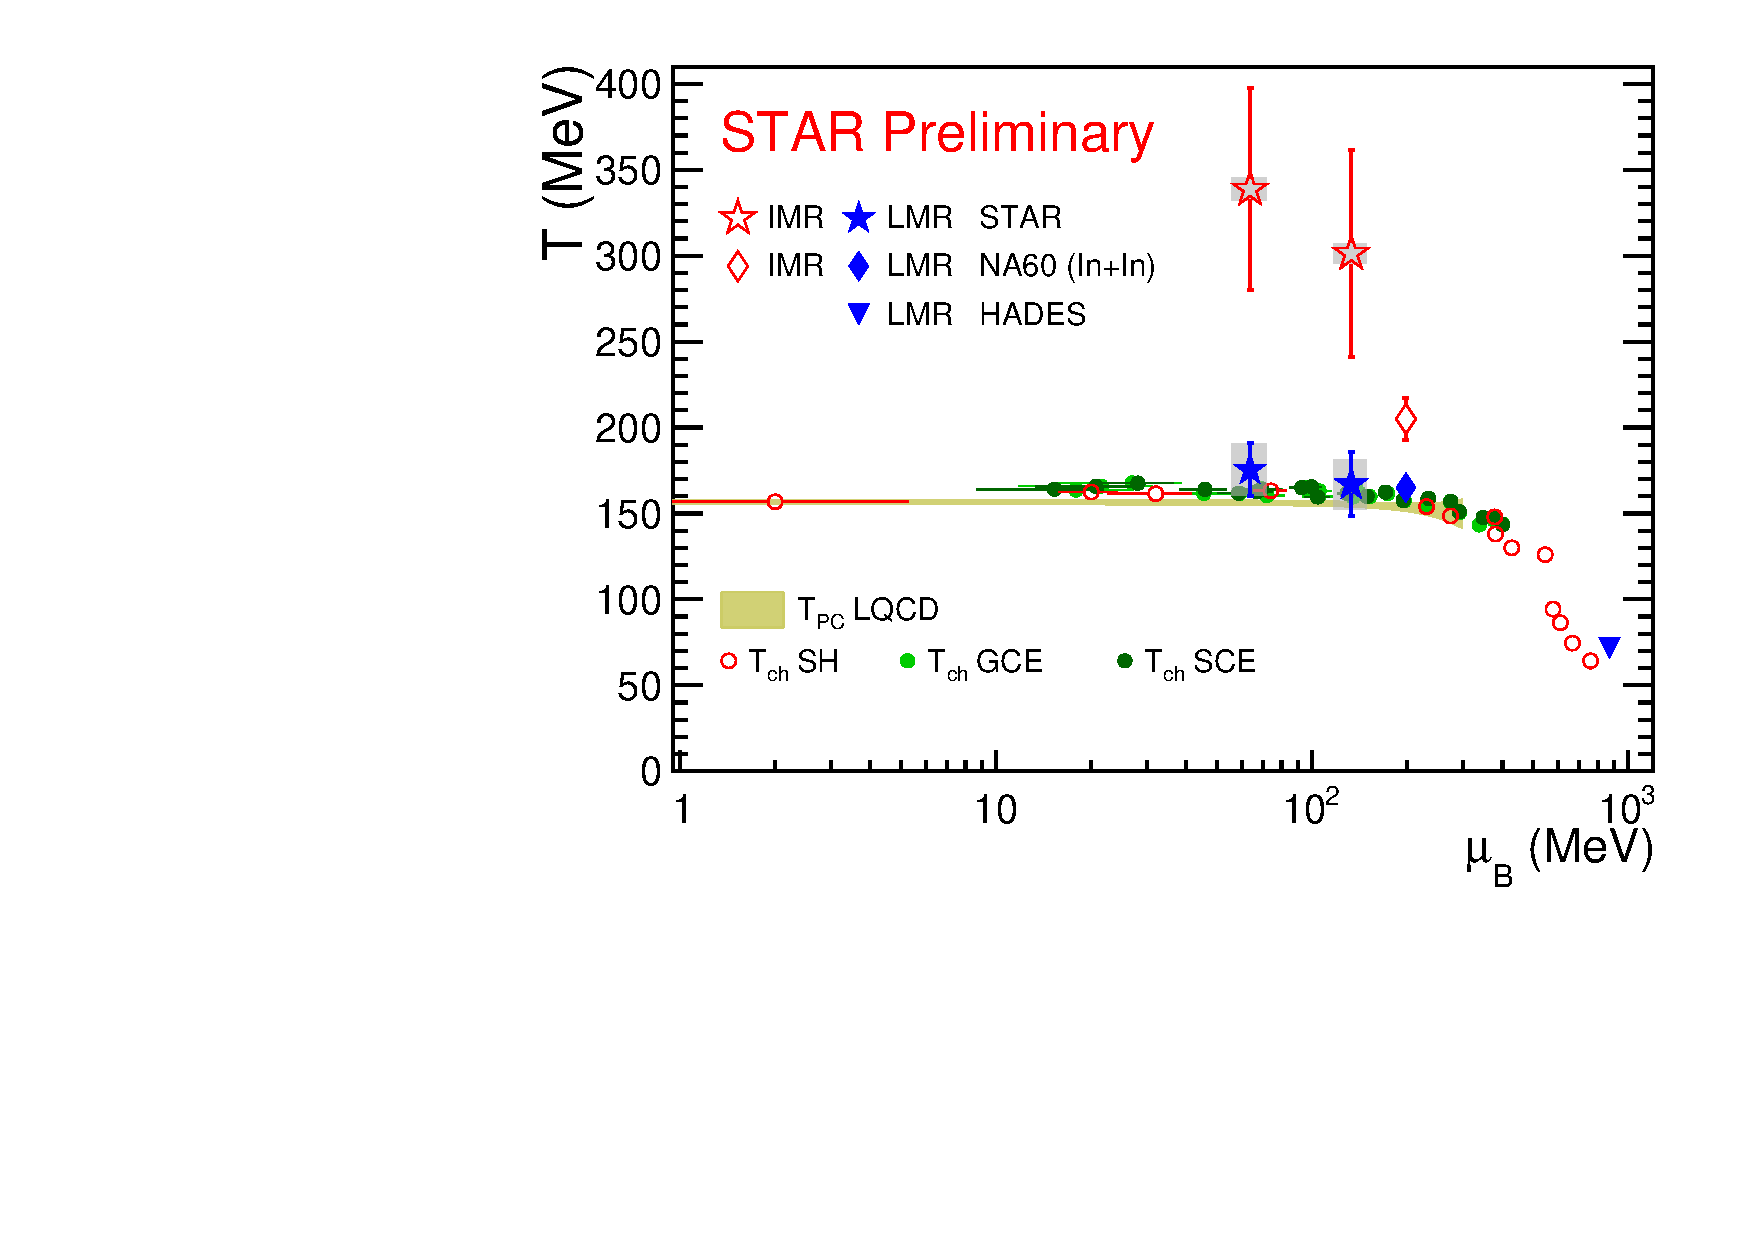
\includegraphics[width=0.75\textwidth,clip]{figures/Chapter4/T_vs_uB_comparedNA60_HADES_phaseTransition_logx_4QM2022.pdf}
    \end{center}
    \caption[双轻子额外产额谱中抽取得到的温度随重子化学势变化示意图]{双轻子额外产额谱中抽取得到的温度随重子化学势变化示意图,图中蓝色的点为在低质量区间的温度抽取结果。红色空心星形和菱形点为在中等质量区间的温度抽取结果。绿色条带为相变温度。绿色数据点和红色空心圆点为化学冻结温度。}
    \label{fig:T_vs_uB_comparedNA60_HADES_phaseTransition_logx_4QM2022}
\end{figure}